The N-Queens puzzle is the problem of placing N chess queens on an NxN
chessboard so that no pair of queens attack each other~\cite{8queens}. The
specific challenge of finding all the distinct solutions to this problem is a
good benchmark in designing parallel algorithms.  Most popular parallel
implementations of the N-Queens problem distribute the search space of the
problem by assigning incomplete boards as tasks to threads.  Our approach is
unusual since we see the squares of the board as the LM's nodes of the program,
where each square can communicate with other 4 squares: the adjacent right and
the adjacent left on the same row, and the first non-diagonal square to the
right and to the left on the row below. To represent a partial/valid board
state, we use a list of integers, where each integers represents the column in
which a queen is placed. For example $[2, 0]$ means that a queen is placed in
square $(0, 0)$ and another in square $(1, 2)$. At any given time, many partial
board states may use the same squares and each square can belong to several
board states. An example final database for the 8-Queens problem is presented in
Fig.~\ref{code:coordination:8queens}, where only 8 valid states of the possible
92 states are shown.

Figure~\ref{code:coordination:nqueens} presents our solution. The predicates
\code{left}, \code{right}, \code{down-left} and \code{down-right} represent each
square's four connections to the squares on the same row and to the row below.
Predicate \code{coord} represents the coordinate of the given square.
Predicates \code{propagate-left} and \code{propagate-right} propagate a given
board state to the left or to the right in the current row of the board.
Predicates \code{test-y}, \code{test-diag-left} and \code{test-diag-right} take
one valid board state (last argument) and then determine if the current square
is able to add itself to that state by checking the three restrictions of the
N-Queens puzzle. Predicate \code{new-state} represent a new valid board state in
the current square, while \code{send-down} forces a square to send a new state
to the squares in the row below. Finally, predicate \code{final-state}
represents a full board state. Once the program completes, the last row of
squares of the board should have several \code{final-state} facts which
represent all the distinct solutions to the puzzle.

In terms of facts and rules, we have an initial fact that represents an empty
state (line~\ref{line:coord:queens_axiom}), which is instantiated in the
top-left square and must be propagated to all squares in the same row (rule in
lines~\ref{line:coord:queens_propr1}-\ref{line:coord:queens_propr2}). If a
square $S$ receives a new state $L$, it checks if $S$ can be incorporated into
$L$. For that, it checks if there is no queen on $S$'s column (rules in lines
\ref{line:coord:queens_col1}-\ref{line:coord:queens_col2}), if there is no queen
on $S$'s left diagonal (rules in
lines~\ref{line:coord:queens_ldiag1}-\ref{line:coord:queens_ldiag2}) and if
there is no queen on $S$'s right diagonal (rules in
lines~\ref{line:coord:queens_rdiag1}-\ref{line:coord:queens_rdiag2}).

\begin{figure}[h!]
\begin{Verbatim}[numbers=left,fontsize=\scriptsize,commandchars=\*\#\&]
type list int state.*hfill// Type declaration
type left(node, node).  type right(node, node).*hfill// Predicate declaration
type down-left(node, node).  type down-right(node, node).
type coord(node, int, int).
type linear propagate-left(node, state).
type linear propagate-right(node, state).
type linear test-y(node, int, state, state).
type linear test-diag-left(node, int, int, state, state).
type linear test-diag-right(node, int, int, state, state).
type linear new-state(node, state).
type linear send-down(node, state).
type linear final-state(node, state).

propagate-left(A, State)*hfill// Rule 1: propagate to the left
  -o {L | !left(A, L), L <> A -o propagate-left(L, State)}, new-state(A, State).
propagate-right(A, State)*label#line:coord:queens_propr1&*hfill// Rule 2: propagate to the right
  -o {R | !right(A, R), R <> A -o propagate-right(R, State)}, new-state(A, State).*label#line:coord:queens_propr2&

new-state(A, State), !coord(A, X, Y) -o test-y(A, Y, State, State).*hfill// Rule 3: check if queen can be added

// check if there is no queen on the same column*label#line:coord:queens_col1&
test-y(A, Y, [], State), !coord(A, OX, OY)*hfill// Rule 4: check vertical
  -o test-diag-left(A, OX - 1, OY - 1, State, State).
test-y(A, Y, [Y1 | RestState], State), Y = Y1*hfill// Rule 5: check vertical
  -o 1. // fail*label#line:coord:queens_empty1&
test-y(A, Y, [Y1 | RestState], State), Y <> Y1*hfill// Rule 6: check vertical
  -o test-y(A, Y, RestState, State).*label#line:coord:queens_col2&

// check if there is no queen on the left diagonal*label#line:coord:queens_ldiag1&
test-diag-left(A, X, Y, _, State), X < 0 || Y < 0, !coord(A, OX, OY)*hfill// Rule 7: check left diagonal
  -o test-diag-right(A, OX - 1, OY + 1, State, State).
test-diag-left(A, X, Y, [Y1 | RestState], State), Y = Y1*hfill// Rule 8: check left diagonal
  -o 1. // fail*label#line:coord:queens_empty2&
test-diag-left(A, X, Y, [Y1 | RestState], State), Y <> Y1*hfill// Rule 9: check left diagonal
  -o test-diag-left(A, X - 1, Y - 1, RestState, State).*label#line:coord:queens_ldiag2&

// check if there is no queen on the right diagonal*label#line:coord:queens_rdiag1&
test-diag-right(A, X, Y, [], State), X < 0 || Y >= size, !coord(A, OX, OY)*hfill// Rule 10: check right diagonal
  -o send-down(A, [OY | State]). // add new queen*label#line:coord:queens_add&
test-diag-right(A, X, Y, [Y1 | RestState], State), Y = Y1*hfill// Rule 11: check right diagonal
  -o 1. // fail*label#line:coord:queens_empty3&
test-diag-right(A, X, Y, [Y1 | RestState], State), Y <> Y1*hfill// Rule 12: check right diagonal
  -o test-diag-right(A, X - 1, Y + 1, RestState, State).*label#line:coord:queens_rdiag2&

send-down(A, State), !coord(A, size - 1, _)*label#line:coord:queens_complete1&*hfill// Rule 13: final state
  -o final-state(A, State).*label#line:coord:queens_complete2&
send-down(A, State), !coord(A, CX, _), CX <> size - 1*label#line:coord:queens_down1&*hfill// Rule 14: propagate the state down
  -o {B | !down-right(A, B), B <> A -o propagate-right(B, State)},
     {B | !down-left(A, B), B <> A -o propagate-left(B, State)}.*label#line:coord:queens_down2&

propagate-right(@0, []).*label#line:coord:queens_axiom&*hfill// Initial fact
\end{Verbatim}
  \mycap{N-Queens problem solved in LM.}
  \label{code:coordination:nqueens}
\end{figure}

If there is any conflict, we do not derive anything and for that we use the
language expression \code{1}
(lines~\ref{line:coord:queens_empty1},~\ref{line:coord:queens_empty2}
and~\ref{line:coord:queens_empty3}). If there are no conflicts, this means that
it is possible to add a queen to the current state
(line~\ref{line:coord:queens_add}). The fact \code{send-down} is used to either
complete the computation of a valid state
(lines~\ref{line:coord:queens_complete1}-\ref{line:coord:queens_complete2}) or
to propagate the state to the row below
(lines~\ref{line:coord:queens_down1}-\ref{line:coord:queens_down2}) as shown in
Fig.~\ref{coordination:fig:nqueens}.
The full proof of correctness for
the N-Queens program is presented in Appendix~\ref{appendix:proofs:nqueens}.

\begin{figure}[h!]
\begin{Verbatim}[numbers=left,fontsize=\codesize,commandchars=\*\#\&]
final-state(@57, [0, 4, 7, 5, 2, 6, 1, 3]).*hfill// States at square (7, 0)
final-state(@57, [0, 5, 7, 2, 6, 3, 1, 4])
final-state(@57, [0, 6, 3, 5, 7, 1, 4, 2])
final-state(@57, [0, 6, 4, 7, 1, 3, 5, 2])

(...)

final-state(@63, [7, 1, 3, 0, 6, 4, 2, 5])*hfill// States at square (7, 7)
final-state(@63, [7, 1, 4, 2, 0, 6, 3, 5])
final-state(@63, [7, 2, 0, 5, 1, 4, 6, 3])
final-state(@63, [7, 3, 0, 2, 5, 1, 6, 4])
\end{Verbatim}
  \mycap{Final database for the 8-Queens program.}
  \label{code:coordination:8queens}
\end{figure}

Since computation goes from the top row to the bottom row, not all static
placements of nodes to threads will perform equally well. This is especially
true because the bottom rows perform the most work.  The best placement is then
to split the board vertically with axiom \code{set-thread(A, vertical(X, Y,
side, side))} so each thread gets the same number of columns, where
\code{vertical} is a function that accepts the coordinates \code{X} and \code{Y}
and the \code{size} of the board and then returns the thread for node \code{A}.
Our experiments show that, on a shared memory system, it does not matter much if
we start with a bad placement since node stealing overcomes those issues by load
balancing dynamically.

\begin{figure}[ht!]
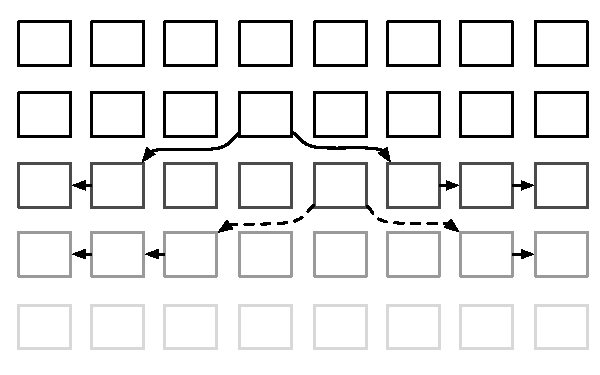
\includegraphics[width=0.4\textwidth]{figures/coordination/nqueens.pdf}
\mycap{Propagation of states using the \code{send-down} fact.}
\label{coordination:fig:nqueens}
\end{figure}

However, the N-Queens program incrementally builds and shares lists representing
valid board states that are transmitted from top to bottom. In order to improve
memory locality, we should then manipulate board states that share a significant
number of elements because each board state needs to be iterated before being
extended with a new position. To accomplish this, we used the coordination fact
\code{set-default-priority(A, X)} (not shown in
Fig.~\ref{code:coordination:nqueens}) to experiment with two main
configurations: \textbf{Top}, where top rows are prioritized; and
\textbf{Bottom}, where squares closer to the bottom are computed first. We also
decided to optionally pin nodes to threads, as mentioned earlier, to see if
memory locality affects the multi-threaded performance of the program. These
configurations are refered as \textbf{Static}.

The complete results are shown in
Fig.~\ref{fig:coordination:results_queens-13} (for the 13-Queens problem) and
Fig.~\ref{fig:coordination:results_queens-14} (for the 14-Queens problem). We
present the 4 possible configurations side by side and compare their run time
against the version without coordination. The line \textbf{Regular(1)/Config(t)}
represents the speedup of the configuration \textbf{Config} against the run
time of the regular version (no coordination) using 1 thread.

The first observation is that using the \textbf{Top} configuration for a small
number of threads results in better run times (see
Fig.~\ref{fig:coordination:results_queens-14}(a) for an example), however that
advantage is lost when adding more threads. We argue that \textbf{Top} allows
threads to build all the valid states on row $i$ and then process them all at
once on row $i+1$, improving overall memory locality since LM rules run for all
possible board configurations of row $i$. However, when the number of threads
increases, it results in reduced scalability since there is less work available
per thread since row $i$ must be processed before row $i+1$.

In the \textbf{Bottom} configuration, there is little change when compared to
the uncoordinated version of N-Queens. However, interesting things happen in the
\textbf{Bottom Static} configuration when the number of rows is equal to the
number of threads. For an example, observe
Fig.~\ref{fig:coordination:coord_14queensbottomstatic} where using 14 threads
takes almost the same run time as the regular version when using 32 threads.  In
this case, each thread is assigned a single column of the chess board and is
able to process only the states for that particular column. This behaviour was
investigated in the Valgrind's CacheGrind tool, which showed that this
particular combination has the smallest number of cache misses. This indicates
that it is helpful to match the problem to the number of available CPU's in the
system in order to increase memory locality.


\begin{figure}[]
        \centering
        \begin{subfigure}[b]{\plotsize\textwidth}
           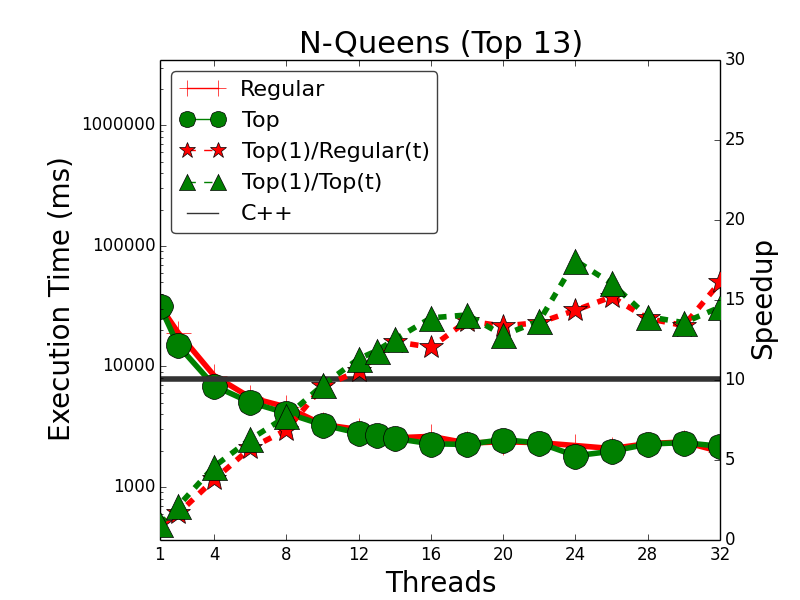
\includegraphics[width=\textwidth]{experiments/coordination/cmp-top-8queens-13.png}
           \mycap{}
           \label{fig:coordination:coord_13queenstop}
        \end{subfigure}
        ~
        \begin{subfigure}[b]{\plotsize\textwidth}
           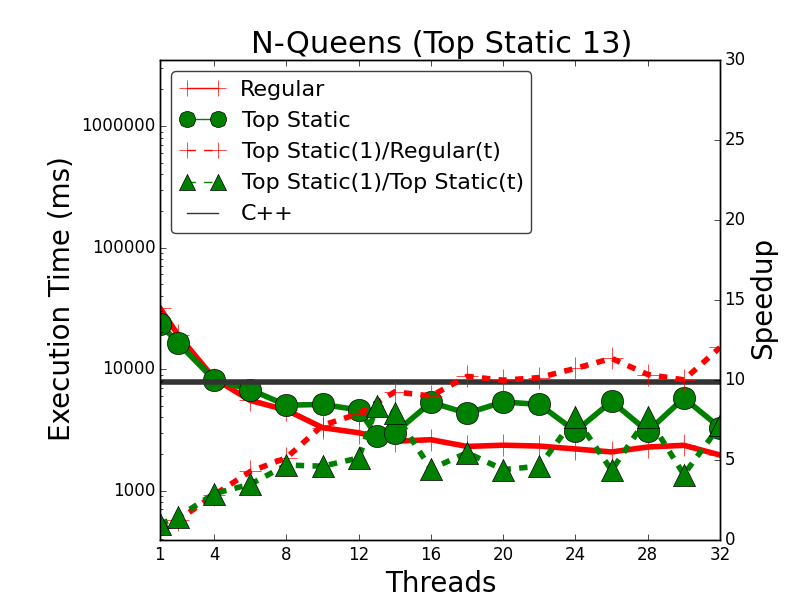
\includegraphics[width=\textwidth]{experiments/coordination/cmp-top-static-8queens-13.png}
           \mycap{}
           \label{fig:coordination:coord_13queenstopstatic}
        \end{subfigure} \\
        \begin{subfigure}[b]{\plotsize\textwidth}
           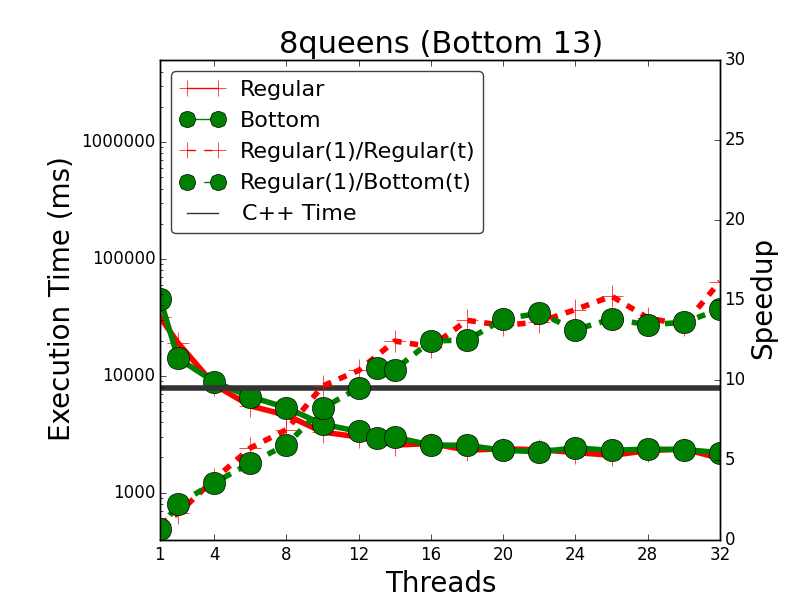
\includegraphics[width=\textwidth]{experiments/coordination/cmp-bottom-8queens-13.png}
           \mycap{}
           \label{fig:coordination:coord_13queensbottom}
        \end{subfigure} ~
        \begin{subfigure}[b]{\plotsize\textwidth}
           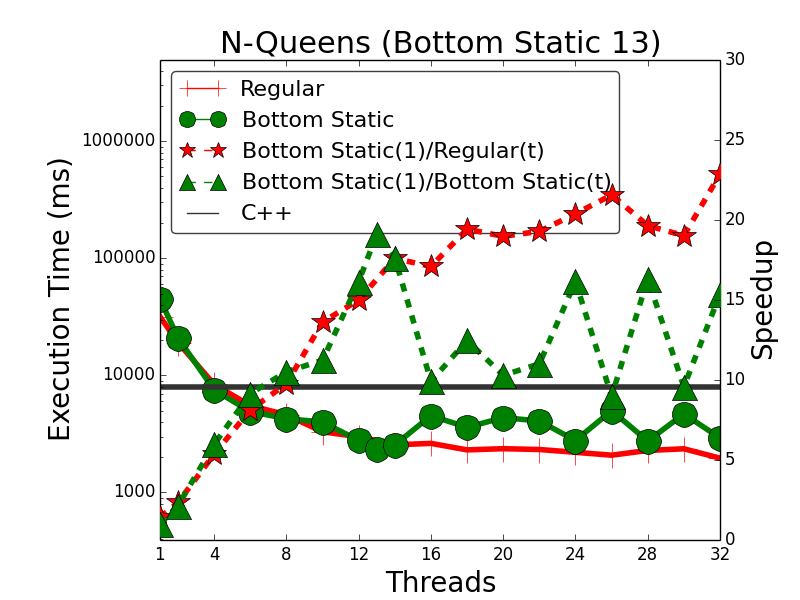
\includegraphics[width=\textwidth]{experiments/coordination/cmp-bottom-static-8queens-13.png}
           \mycap{}
           \label{fig:coordination:coord_13queensbottomstatic}
        \end{subfigure} \\
        \mycap{Scalability for the N-Queens 13 program when using different
        scheduling and partitioning policies.}
        \label{fig:coordination:results_queens-13}
\end{figure}

\begin{figure}[]
        \centering
        \begin{subfigure}[b]{\plotsize\textwidth}
           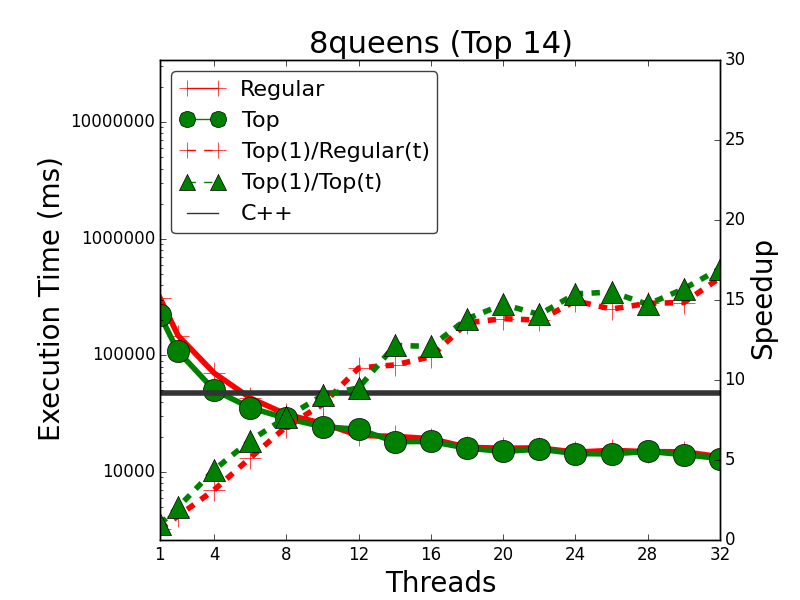
\includegraphics[width=\textwidth]{experiments/coordination/cmp-top-8queens-14.png}
           \mycap{}
           \label{fig:coordination:coord_14queenstop}
        \end{subfigure}
        ~
        \begin{subfigure}[b]{\plotsize\textwidth}
           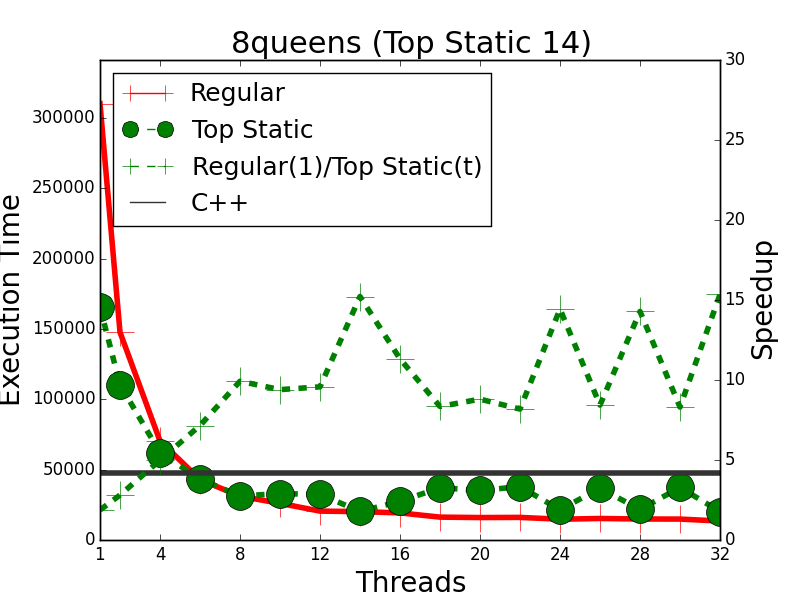
\includegraphics[width=\textwidth]{experiments/coordination/cmp-top-static-8queens-14.png}
           \mycap{}
           \label{fig:coordination:coord_14queenstopstatic}
        \end{subfigure} \\
        \begin{subfigure}[b]{\plotsize\textwidth}
           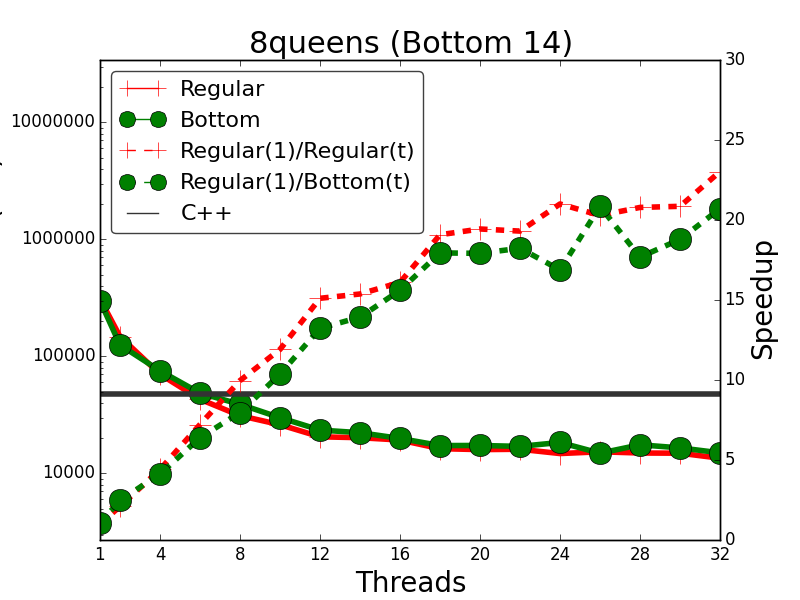
\includegraphics[width=\textwidth]{experiments/coordination/cmp-bottom-8queens-14.png}
           \mycap{}
           \label{fig:coordination:coord_14queensbottom}
        \end{subfigure} ~
        \begin{subfigure}[b]{\plotsize\textwidth}
           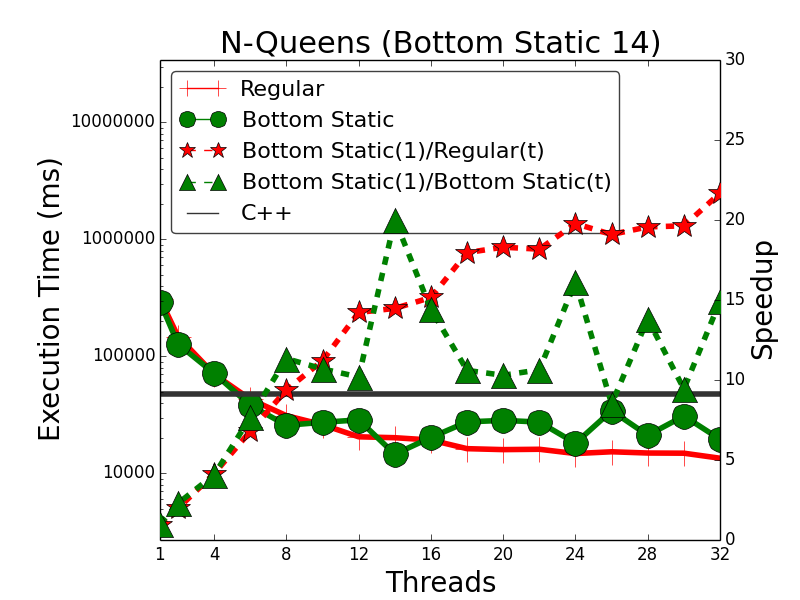
\includegraphics[width=\textwidth]{experiments/coordination/cmp-bottom-static-8queens-14.png}
           \mycap{}
           \label{fig:coordination:coord_14queensbottomstatic}
        \end{subfigure} \\
        \mycap{Scalability for the N-Queens 14 program when using different
        scheduling and partitioning policies.}
        \label{fig:coordination:results_queens-14}
\end{figure}

%We prove that the N-Queens program finds all the distinct solutions for the
puzzle. In the following lemmas, we assume that $(X_0, Y_0)$ is the coordinate
of square/node $A$.

\begin{lemma}[test-y lemma]

From a fact \code{test-y}$(A, Y, State, OrigState)$, there are two possible
scenarios:

\begin{itemize}
   \item The \code{test-y} fact and everything derived from it is retracted and
      there is a coordinate $(X', Y) \in State$.
   \item The \code{test-y} fact is retracted and is used to derive a
      \code{test-diag-left}$(A, X_0 - 1, Y_0 - 1,
      OrigState, OrigState)$ fact since 
      there is no such coordinate $(X', Y) \in State$.
\end{itemize}

\end{lemma}
\begin{proof}
Induction on the size of \code{State}.

First rule: immediately the second scenario.

Second rule: immediately the first scenario.

Third rule: by induction.
\end{proof}

\begin{lemma}[test-diag-left lemma]
   From a fact \code{test-diag-left}$(A, X, Y, State, OrigState)$, there are
  two possible scenarios:
   
  \begin{itemize}
     \item The \code{test-diag-left} fact and everything derived from it is
        retracted and there is a coordinate $(x', y') \in State$, where $x' = X
        - a$ and $y' = Y - a$, where $a$ is non-negative.
     \item The \code{test-diag-left} is retracted and is used to derive a
        \code{test-diag-right}$(A, X_0 - 1, Y_0 + 1, OrigState, OrigState)$
        fact since there is no $(x', y')$ coordinate as specified above.
  \end{itemize}
\end{lemma}
\begin{proof}
Induction on the size of \code{State}.

First rule: immediately the second scenario.

Second rule: immediately the first scenario.

Third rule: by induction.
\end{proof}

\begin{lemma}[test-diag-right lemma]
From a fact \code{test-diag-right}$(A, X, Y, State, OrigState)$, there are
two possible scenarios:

\begin{itemize}
   \item The \code{test-diag-right} fact and everything derived from it is
      retracted and there is a coordinate $(x', y') \in State$, where $x' = X -
      a$ and $y' = Y + a$, where $a$ is non-negative.
   \item The \code{test-diag-right} fact is retracted and the fact
      \code{send-down}$(A, [(X_0, Y_0) | OrigState])$ is derived.
\end{itemize}
\end{lemma}

\begin{proof}
Induction on the size of \code{State}.

First rule: immediately the second scenario.

Second rule: immediately the first scenario.

Third rule: by induction.
\end{proof}

\begin{theorem}[State validation]
From a fact \code{test-y}$(A, Y_0, State, State)$, there are two possible
scenarios:
   
   \begin{itemize}
      \item The \code{test-y} fact and anything derived from it is retracted.
      \item The \code{test-y} fact is retracted and a \code{send-down}$(A,
         [(X_0, Y_0) | State])$ fact is derived, where $[(X_0, Y_0) | State]$ is
         a valid board state.
   \end{itemize}
\end{theorem}
\begin{proof}
Use the previous three lemmas.
\end{proof}

\begin{lemma}[Propagate left lemma]
If a \code{propagate-left}$(A, State)$ fact exists then every cell to the left,
including \code{A} will derive \code{new-state(A, State)}. The original
\code{propagate-left} fact and any other fact derived from it (except
\code{new-state}) are retracted.
\end{lemma}
\begin{proof}

By induction on the number of cells to the left of $A$ and using the only rule
that uses \code{propagate-left}.

\end{proof}

\begin{lemma}[Propagate right lemma]
If a \code{propagate-right}$(A, State)$ fact exists then every cell to the left,
including \code{A} will derive \code{new-state(A, State)}. The original
\code{propagate-right} fact and any other fact derived from it (except
\code{new-state}) are retracted.
\end{lemma}
\begin{proof}
By induction on the number of cells to the left of $A$ and using the only rule
that uses \code{propagate-right}.
\end{proof}

\begin{theorem}[States theorem]
For a given row, we compute several \code{send-down}$(A, State)$ facts that
represent valid states that include that row and the rows above.
\end{theorem}
\begin{proof}
By induction on the number of rows.

For row 0, we use the initial fact \code{propagate-right}$(\mathtt{@0}, [])$,
that will be propagated to all nodes in row 0 (propagate right lemma). By using
the state validation theorem, we know that every node will derive
\code{send-down(A, [(X, Y)])}, which are all the valid states.

By induction, we know that row $X'$ has derived every \code{send-down} fact
possible. Such facts will be sent downwards to row $X = X' + 1$ using the last
rule in the program, deriving \code{propagate-right} or \code{propagate-left}
that, in turn, will derive a \code{new-state} fact at each right or left square.
Nothing is derived at the square below or the diagonal cells since they are not
valid.  From the \code{new-state} fact, a \code{test-y} fact is derived, which will be
checked using the state validation theorem, filtering all new valid
states and then finally deriving a new \code{send-down} fact.

\end{proof}


\clearpage
